\documentclass{article}
%
%babel
\usepackage[romanian]{babel}
%
\usepackage{graphicx}%dorim să importăm grafică
\usepackage{amsfonts}
\title{Evoluţia stelelor}
\author{Predescu Theodor\footnote{313AC}}
\date{}
\begin{document}
\maketitle
\begin{abstract}
Rezumat. Acest articol conţine informaţii utile pentru profesorii de fizică din gimnaziu privind studiul stelelor şi evoluţia lor. De asemenea, conţine link-uri către curriculum tipic pentru şcoală şi sugerează activităţi relevante pentru elevi.
\end{abstract}
%
\section{Introducere}\label{intro}
	Evoluţia stelară presupune orice modificare apărută la nivelul stelelor, începând cu naşterea acestora, de-a lungul vieţii lor îndelungate şi până la moarte, de la ,,Forţele" gravitaţionale ale stelelor la energia radiantă. Pentru a compensa această pierdere de energie, stelele produc energie prin procese de fuziune nucleară a unor elemente uşoare în altele mai grele. 
\section{Obiective}
	Un obiectiv principal în astronomie este determinarea puterii stelelor de diferite tipuri. Așadar, în cazul în care se observă un anumit tip de stea într-o parte a Universului, astronomii pot să utilizeze luminozitatea B şi puterea presupusă P pentru a determina distanţa D pătratului invers a luminozităţii (1).
\begin{equation}
	B\sim\frac{P}{D}
\end{equation}
	Temperatura unei stele se poate determina şi cu ajutorul spectrului său – distribuţia culorilor sau a lungimilor de undă a luminii stelei. Această figură ilustrează frumuseţea culorilor luminii stelelor. Această lumină a trecut de atmosfera exterioară a stelei, şi ionii, atomii şi moleculele din atmosferă îndepărtează anumite lungimi de undă din spectru.
\begin{table}[htbp]
\centering
\caption{Unități de măsura}\label{tab:unit}
\begin{tabular}{lllll}
\hline
Nr.&Clasa&Culoare conventionala&Masa&Linii de Hidrogen\\\hline
1 &O&albastru&60M&slabe\\\hline
2&B &alb-albastre*18M&medii\\\hline
3&A&alb&3.1M&puternice\\\hline
4&F&alb-galbui&1.7M&medii
\end{tabular}
\end{table}
Pentru raportul atomic al unui element „E" în raport cu hidrogenul (H). Uneori simbolul elementului este luat ca prescurtare pentru a exprima numărul de atomi, n(E). \ref{fig:figura}...
\begin{figure}[ht]
\centering
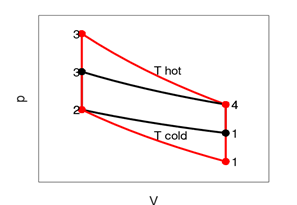
\includegraphics[bb=50 50 50 50]{Picture1.png}
\caption{Grafic ce ilustră scara de ambundență în raport cu creșterea numărului atomic al elementelor}\label{fig:figura}
\end{figure}
\section{Concluzii}
Cu aproximativ un secol în urmă, era studiilor cantitative moderne despre abundența și distribuția elementelor chimice a început, deoarece aproape toate elementele naturale ale tabelului periodic au fost descoperite. Analizele chimice nu se mai limitau la elementele majore care apar în roci, iar mecanica cuantică deschisese ușa analizelor spectrale cantitative ale soarelui și stelelor. A existat și rămâne o puternică dorință de a ști care elemente există și cantitățile lor pe suprafața Pământului, în interiorul Pământului și Planetelor, Soarelui și Cosmosului. Principiile nucleosintetice, geochimice și cosmochimice care guvernează formarea și distribuția elementelor rămân domenii active de cercetare în astrofizică și cosmochimie. În mod tradițional, cunoștințele despre abundența elementară provin din două discipline - astronomie cu studii despre compoziția soarelui și a altor stele și cosmochimie cu studii practice ale meteoriților, interplanetarului și prafului interstelar. Ambele discipline se completează reciproc pentru a valida, completa și optimiza datele despre abundența sistemului solar, care sunt utilizate pe scară largă ca compoziție de referință în ambele discipline.
\begin{thebibliography}{a}
\bibitem{wiki} Wikipedia-Legile lui Newton:

	$\bullet$ Bennett, Jeffrey et al, The Essential Cosmic Perspective, Addison-Wesley; one of the best of the many available textbooks in introductory astr nomy,2005.
	
	$\bullet$ Kaler, James B, The Cambridge Encyclopaedia of Stars, Cambridge Univ. Press, 2006.
	
	$\bullet$ Percy, J.R, Understanding Variable Star, Cambridge University Press, 2007

\end{thebibliography}
\end{document}